\section{Example Repositiories}
\label{sec:review}

In this section, we present two example file repositories.
We will use these examples to help us motivate and explain
the design of \forest{} in future sections.

The first repository contains information about students in
Princeton's undergraduate computer science program.   
The data in the repository is used
every year to help faculty decide on undergraduate awards,
to assign honors levels (honors, high honors, highest honors)
to graduating seniors and to track grading trends.
It was
created in approximately 1990 and has been extended and
maintained ever since.  As the repository has evolved over time, there
have been a few slight changes in format -- a typical occurrence in
ad hoc data repositories.  Naturally, any description will need to cope
with the variation.
 
Figure~\ref{fig:student-pic} shows the
structure of the student data repository.  At the top level, there are
three important directories: \cd{graduates} (students who have graduated)
\cd{classof11} (this year's seniors) and \cd{classof12} (this year's juniors).
There is also a \cd{README} file containing a collection of notes.
Inside \cd{graduates}, there is another set of directories named 
\cd{classofX} where \cd{X} dates back to 92.  Inside each \cd{classofX} 
directory, there are at least the 
two degree subdirectories \cd{ABX} and \cd{BSEX} as
the computer science department gives out both Arts and Science
and Engineering degrees.  Optionally, there are also subdirectories for
students who left Princeton or transferred into another program. 
Within any degree subdirectory, there is a set of text files, one
textfile per student, that contain information on courses taken and
student grades.  Figure~\ref{fig:student-file-example} present a fragment
of a typical file.  The directory also usually contains a blank template file
named \cd{sss.txt} or something similar for creating new students.

\begin{figure}

a picture showing the student hierarchy

\caption{Princeton computer science undergraduate data.}
\label{fig:student-pic}
\end{figure}

\begin{figure}
% Note: Kessel has poor grades in COS but excels in HOC and 
% is taking a grad course in GOL(s).  :-)
\begin{code}
KESSEL, PHIL	   BSE   '11
- - - - - - - - - - - - - - - - - - -
Type    Yr  Course     Grade
         1             A+ to F
d        2             P  (  Pass )
t  D  p  3             INC
o  .  .  4  Dept  xxx  N  (Not Avail)
- - - - - - - - - - - - - - - - - - -
d  .  .  1  COS   101  C
o  .  .  1  HOC   101  A
o  .  .  1  GOL   599  A+
...
\end{code}
\caption{Example student file {\tt KESSEL.txt}.}
\label{fig:student-file-example}
\end{figure}

The second repository contains log files for the Coral Content
Distribution Network
(CoralCDN)~\cite{freedman+:coral,freedman:coral-experience}. To
monitor the performance, health, and security of the system, the hosts
participating in CoralCDN periodically send statistics reports back to
a central server. These statistics are collected up and stored in a
directory similar to the one depicted in Figure~\ref{fig:coral-pic}.
The top-level \cd{log} directory contains a set of subdirectories, one
for each host. Each host directory contains another set of
directories, labeled by date and time. Finally, each of these
directories contains one or more compressed log files. For the
purposes of this example, we will focus on the \cd{coralwebsrv.log.gz}
log file, which contains detailed information about the web requests
made on the host during the preceding time period.

\reminder{We should check with Mike that including this information (machine
  names, dates) is okay. Also, we will probably need to make
  the graph smaller by eliding some nodes.}

\begin{figure}
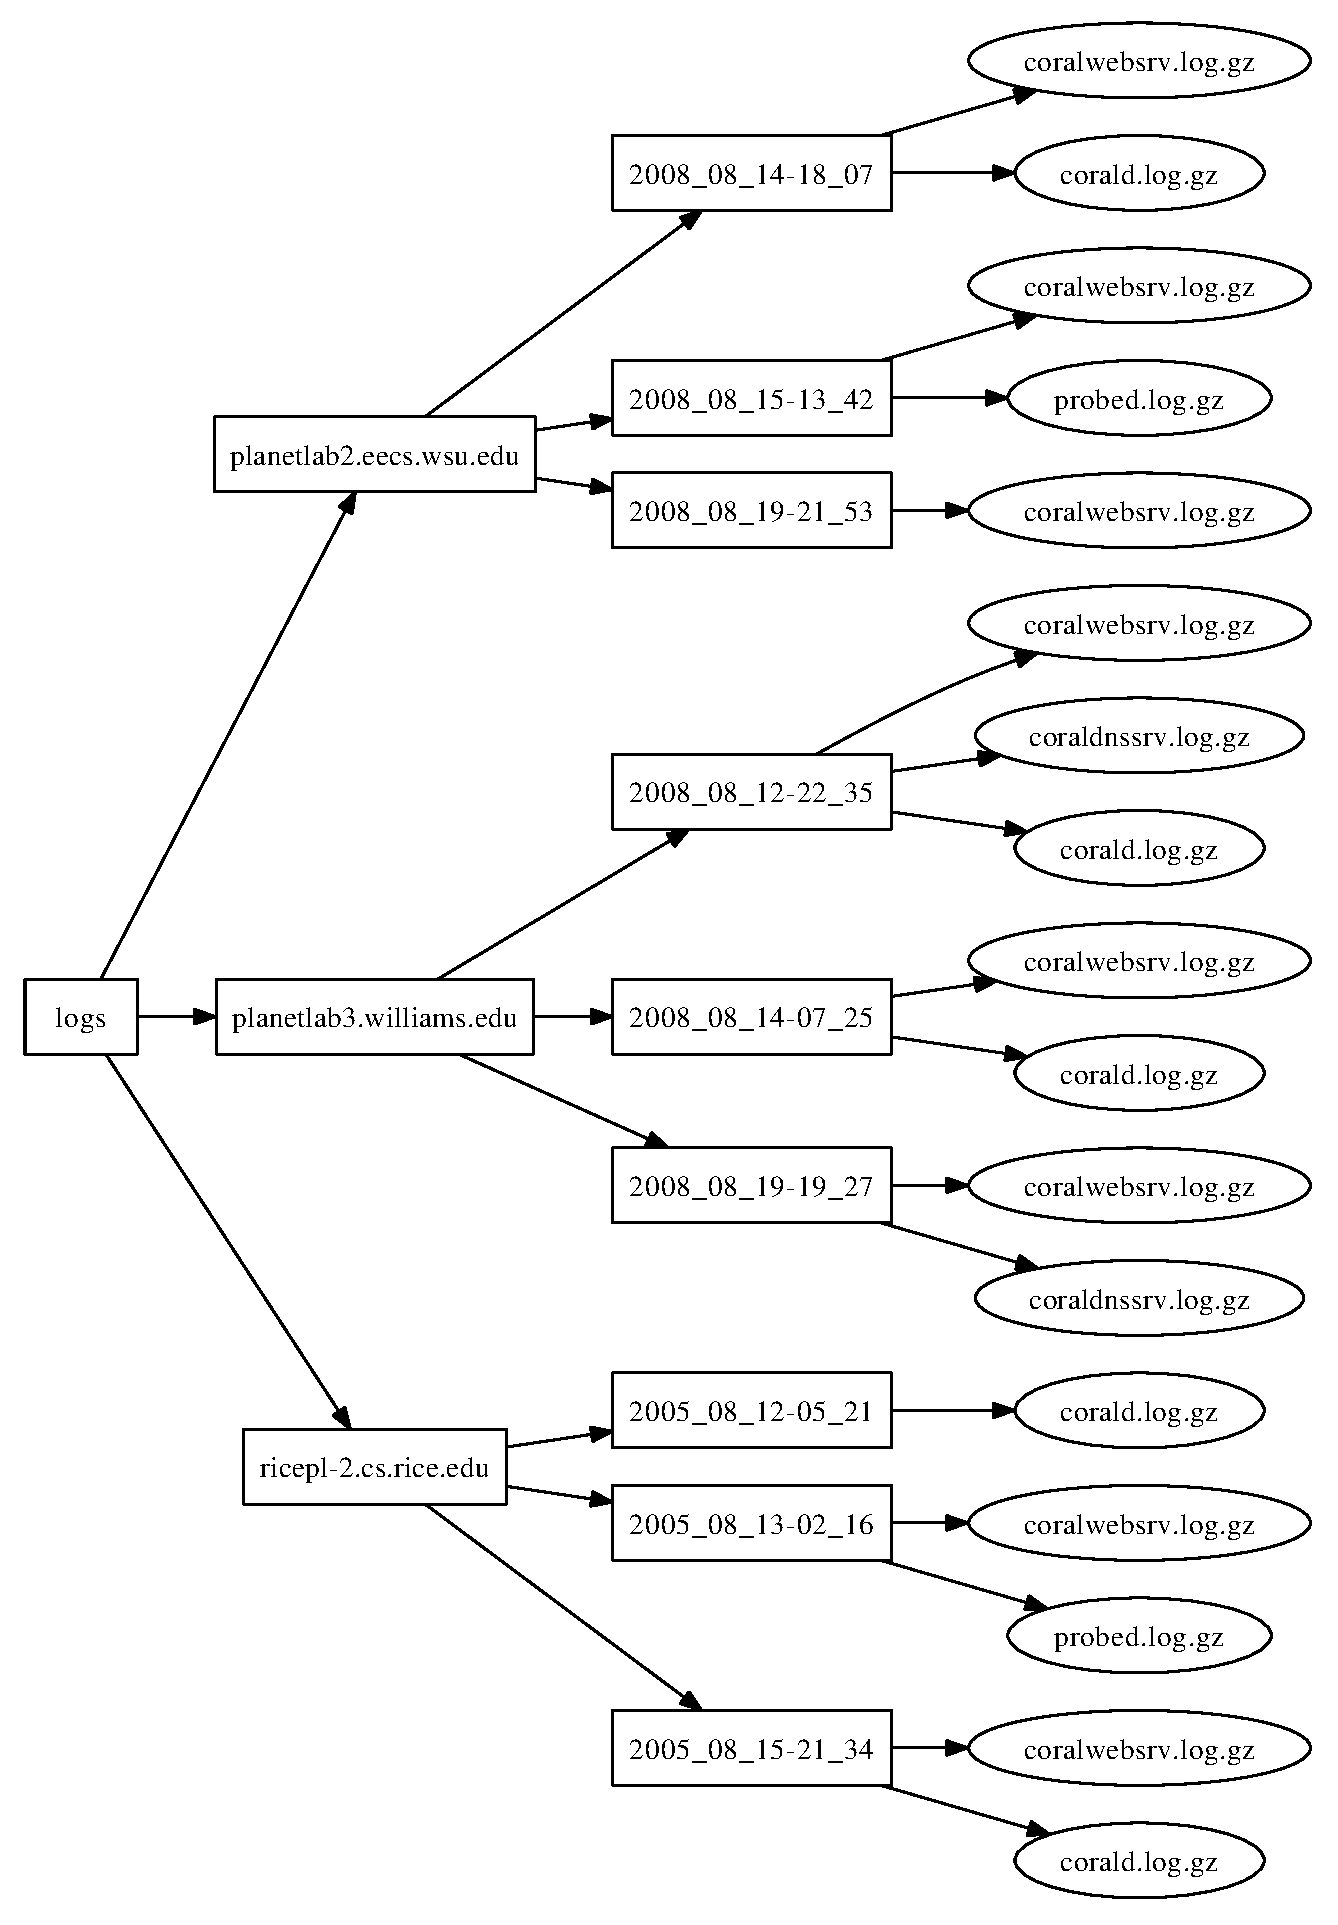
\epsfig{file=coral-structure.eps, width=0.9\columnwidth}
\caption{Coral system log data.}
\label{fig:coral-pic}
\end{figure}

